%\yoc{I strengthened this section towards discussing why the things we consider are important. }
In this section, we explain information about the test problems included in \siplibtwo\ in a summarized manner. This includes problem origin, type, components (variables and constraints), and sparsity for each problem. We discuss why they are important for advances in SIP research study. This section also reflects our philosophy in developing \siplibtwo. Detailed problem-specific explanation is available in Section \ref{sec:prob_desc} for those who are interested in.

\subsection{Origin of the problems}
Table \ref{table:problems} summarizes the description of each test problem in \siplibtwo. The nine of them (except \sdcp\ and \suc) are adopted from existing libraries, Shabbir Ahmed's \siplib\ \cite{web:SIPLIB1} and Andy Felt's test-problem collection for stochastic linear programming \cite{journal:AF2004}. We tried to implement the problems as the same as the original references possible. Not all of them, however, are exactly the same mainly due to insufficient information. We sometimes needed to guess the missing links and develop our own way to implement the problems. 


	
\begin{table}[H]
	\centering
%	\resizebox{\textwidth}{!}{%
			\caption{Problems in \siplibtwo}
			\label{table:problems}
			\begin{tabular}{@{}llll@{}}
				\toprule
				Problem		  		  & Description                                                        & Main reference              \\ \midrule
				\airlift\ & Airlift operations scheduling (\ref{AIRLIFT}) & Midler and Wollmer \cite{journal:MW1969} \\
				\cargo\ & Cargo network scheduling (\ref{CARGO}) & Mulvey and Ruszczy\`{n}ski \cite{journal:MR1995}\\
				\chem\ & Design of batch chemical plants (\ref{CHEM}) & Subrahmanyam et al. \cite{journal:SPR1994}\\				
				\dcap\         & \makecell[tl]{Dynamic capacity planning with stochastic\\ demand (\ref{DCAP}) }                  & Ahmed and Garcia \cite{journal:AG2004}                          \\
				\mptsps\       & \makecell[tl]{Multi-path traveling salesman problem with\\ stochastic travel costs (\ref{MPTSPs})}& Tadei et al. \cite{journal:TPP2017}                            \\
				\phone\       & Telecommunication network planning (\ref{PHONE})& Sen et al. \cite{journal:SDC1994}                            \\
				\sdcp\ 	& Stochastic data center placement (\ref{SDCP}) & Kim et al. \cite{journal:KYZC2017}\\
				\sizes\        & \makecell[tl]{Optimal product substitution with stochastic\\ demand (\ref{SIZES})}         & Jorjani et al. \cite{journal:JSW1999}          \\
				\smkp\		  & Stochastic multiple knapsack problem (\ref{SMKP})                              & Angulo et al. \cite{journal:AAD2014}                            \\
				\sslp\         & Stochastic server location problem (\ref{SSLP})                                & Ntaimo and Sen \cite{journal:NS2005}                           \\
				\suc\         & Stochastic unit commitment problem	(\ref{SUC})			               & Papavasiliou and Oren \cite{journal:PO2013}                       \\ \bottomrule
			\end{tabular}%
			
			%			\begin{tablenotes}
			%				\small
			%				\item For convenience, we skip the cardinality sign $|\cdot|$ for sets, i.e., for any set $S$, $S$ denotes the number of elements $|S|$ in this table.
			%			\end{tablenotes}
%	}
\end{table}

%\begin{table}[H]
%	\centering
%%	\resizebox{\textwidth}{!}{
%	\caption{Problems in \siplibtwo}
%	\label{table:problems}
%%	\resizebox{\textwidth}{!}{%
%	\begin{tabular}{@{}llp{0.3 \textwidth}}
%		\toprule
%		Problem		  		  & \multicolumn{1}{c}{Description}                                                        & \multicolumn{1}{c}{Main reference}              \\ 
%		\midrule
%		\airlift\ & Airlift operations scheduling (\ref{AIRLIFT}) & Midler and Wollmer \cite{journal:MW1969} \\
%		\cargo\ & Cargo network scheduling (\ref{CARGO}) & Mulvey and Ruszczy\`{n}ski \cite{journal:MR1995}\\
%		\chem\ & Design of batch chemical plants (\ref{CHEM}) & Subrahmanyam et al. \cite{journal:SPR1994}\\				
%		\dcap\         & Dynamic capacity planning with stochastic demand (\ref{DCAP})                   & Ahmed and Garcia \cite{journal:AG2004}                          \\
%		\mptsps\       & Multi-path traveling salesman problem with stochastic travel costs (\ref{MPTSPs}) & Tadei et al. \cite{journal:TPP2017}                            \\
%		\phone\       & Telecommunication network planning (\ref{PHONE})& Sen et al. \cite{journal:SDC1994}                            \\
%		\sdcp\ 	& Stochastic data center placement (\ref{SDCP}) & Kim et al. \cite{journal:KYZC2017}\\
%		\sizes\        & Optimal product substitution with stochastic demand (\ref{SIZES})         & Jorjani et al. \cite{journal:JSW1999}          \\
%		\smkp\		  & Stochastic multiple knapsack problem (\ref{SMKP})                              & Angulo et al. \cite{journal:AAD2014}                            \\
%		\sslp\         & Stochastic server location problem (\ref{SSLP})                                & Ntaimo and Sen \cite{journal:NS2005}                           \\
%		\suc\         & Stochastic unit commitment problem	(\ref{SUC})			               & Papavasiliou and Oren \cite{journal:PO2013}                       \\ 
%		\bottomrule
%	\end{tabular}%
%%	}
%\end{table}

\subsubsection{How we deal with missing links and errors}
%\yoc{This subsection is newely added to discuss the issues on implementaion.}
During implementation, we often faced some missing links and errors. The missing links are largely from the deterministic and random parameters. For example, we could not catch the exact data generating procedure for \mptsps\ even after looking up all the relevant references. For \sslp, the parameters for the zonal constraints are not provided ($Z$, $w_z$, $J_z$ in Table \ref{sslp:notation}). 

We also found some errors. The errors are not critical so the instances provided by the former collections are still solvable somehow. The result, however, might be different from the originally intended. For example, we found from \smps\ files of \dcap\ that the big-M constant in the logical constraint (\ref{dcap:b}) is set to be 1 instead of a suitably large value. For \sslp, the redundant constraint (\ref{sslp:b}) presents in the \smps\ files. 

We set the following rule to address such issues described above.
\begin{enumerate}
	\item Follow the original implementation including the errors whenever we are able to reproduce them.
	\item Develop our own way as long as it does not harm the endemic characteristic of the problem.
\end{enumerate}

The notable remark for each problem briefly presents in Table \ref{table:remarks}.
\begin{table}[H]
	\centering
	\resizebox{\textwidth}{!}{%
		\begin{threeparttable}
			\caption{Implementation remarks for each problem}
			\label{table:remarks}
			\begin{tabular}{@{}lp{0.8\textwidth}}
				\toprule
				Problem & \multicolumn{1}{c}{Remark}                                                \\ \midrule
				\airlift & -\\
				\cargo & We adopt the numerical example provided by \cite{journal:AF2004}. We use an uniform distribution to generate random amount of cargo to be shipped. We add additional constraints (\ref{cargo:k})-(\ref{cargo:m}) to make the model valid.\\
				\chem & We use the same numerical example created in \cite{journal:AF2004}. We use uniform distributions for the random parameters. \\
				\dcap   & We go with the error in constraint (\ref{dcap:b}).                                              \\
				\mptsps & We adopt formulation from another reference \cite{journal:LSD1990}. We develop data generation procedure \ref{mptsps:datagen}. \\
				\phone & We use the same numerical example created in \cite{journal:AF2004}. \\
				\sdcp & We generate and provide up to 1,000 wind scenarios.\\
				\sizes  &  We modify the formulation to polish (\ref{sizes:obj})-(\ref{sizes:h}). We develop data generation procedure.                                                 \\
				\smkp   & -                                                                         \\
				\sslp   & We keep the zonal components empty and let the redundant constraint (\ref{sslp:b}) present.                                     \\
				\suc    & We generate and provide up to 1,000 wind scenarios.                              \\ \bottomrule
			\end{tabular}
			\begin{tablenotes}
				\small
				\item Remark. - means no issue presents
			\end{tablenotes}
		\end{threeparttable}
	}
\end{table}

\subsection{Instance naming rule}
Table \ref{table:naming_rule} shows how we name the instances. We change the original naming convention for consistency and future extension. Some legacy naming rules do not consider the case where the set cardinality becomes larger than 1 digit number. Moreover, since some \siplibtwo\ instances can be generated using more sets than used in \siplib, we needed to define a new naming convention. For example, we change the instance names of \dcap\ and \smkp\ as below.
\begin{quote}
	\centering dcap$RNT$\_$\mathcal{S}$ $\longrightarrow$ DCAP$\_R\_N\_T\_\mathcal{S}$\\
	smkp$\_\mathcal{S}$ $\longrightarrow$ SMKP$\_I\_\mathcal{S}$
\end{quote}
For \dcap, we just add underbars ``\_'' to delimit set cardinalities. Without such a delimiter, the instance name causes confusion when set cardinality is greater than or equal to 10. For \smkp, we add new set cardinality $I$ since the fixed number $|I|=120$ can be changed by user if desired.

The capital letters mean the sets defining the instances. In particular, the calligraphic letter $\mathcal{S}$ always denotes the scenario set. For notational convenience, we sometimes skip the cardinality sign $|\cdot|$ for sets, i.e., for a set $S$, $S$ itself denotes the number of elements $|S|$ in Table \ref{table:naming_rule} and \ref{table:num_components}. Note that not all sets are used to define an instance. The sets that do not appear in the instance name are fixed by some constant values. For example, in \smkp\ there are four sets in total, $I,J,K,\mathcal{S}$, but the numbers of knapsacks $|J|$ and $|K|$ are fixed by 50 and 5 so do not appear in the instance name.

The lowercase letters in the instance names denote the non-set parameters defining the instances. Some of them are numbers and some are strings. For SDCP\_$k$\_$p$\_$d$\_$\mathcal{S}$, for example, $k$ is a positive integer, $p$ is a real number between 0.0 and 100.0, and $d$ is a string that would be chosen as one of the \{``FallWD'', ``FallWE'', ``WinterWD'', ``WinterWE'', ``SpringWD'', ``SpringWE'', ``SummerWD'', ``SummerWE''\}. 
\begin{table}[H]
	\centering
	\caption{Instance naming rules}
	\label{table:naming_rule}
	\resizebox{\textwidth}{!}{%
		\begin{tabular}{@{}llp{0.6\textwidth}}
%		\begin{tabular}{@{}llp{3in}}
			\toprule
			Problem & Instance name                 & \multicolumn{1}{c}{Remark}                                                                    					      \\ \midrule
			\airlift	& AIRLIFT\_$\mathcal{S}$& $\mathcal{S}$: number of scenarios\\
			\cargo	& CARGO\_$\mathcal{S}$& $\mathcal{S}$: number of scenarios\\		
			\chem	& CHEM\_$\mathcal{S}$& $\mathcal{S}$: number of scenarios\\				
			\dcap\    & DCAP\_$R$\_$N$\_$T$\_$\mathcal{S}$    &   $R$: number of resources, $N$: number of tasks, $T$: number of time periods, $\mathcal{S}$: number of scenarios        \\
			\mptsps\  & MPTSPs\_$d$\_$N$\_$\mathcal{S}$ &$d$: node distribution strategy, $N$: number of nodes, $\mathcal{S}$: number of scenarios\\
			\phone	& PHONE\_$\mathcal{S}$& $\mathcal{S}$: number of scenarios\\
			\sdcp\ & SDCP\_$k$\_$p$\_$d$\_$\mathcal{S}$ & $k$: maximum number of dispatchable loads, $p$: wind penetration level (\%), $d$: day type, $\mathcal{S}$: number of scenarios\\
			\sizes\   & SIZES\_$\mathcal{S}$                            & $\mathcal{S}$: number of scenarios   															\\
			\smkp\    &   SMKP\_$I$\_$\mathcal{S}$    &   $I$: number of types for item, $\mathcal{S}$: number of scenarios  													 \\
			\sslp\    &  SSLP\_$I$\_$J$\_$\mathcal{S}$      &    $I$: number of clients, $J$: number of server locations, $\mathcal{S}$: number of scenarios                 				   \\
			\suc\    & 	SUC\_$d$\_$\mathcal{S}$    &  $d$: day type, $\mathcal{S}$: number of scenarios                                                 						 \\ \bottomrule
		\end{tabular}%
	}
\end{table}

\subsection{Type of the problems}
In \siplibtwo\, we mainly classify each problem by its stage-wise variable types. Many decomposition-based solution methods in SIP require specific type of variables to be presented in each stage, e.g., \cite{journal:LL1993,journal:SSV1998,journal:CT1998,journal:CS1999,journal:SF2002}. They oftentimes exploit the characteristics of the variables to extend the existing decomposition methods. Therefore, the stage-wise variable type is one of the most important factor that defines SIP problems.

We consider three types of variable: continuous, binary, and integer. Considering two stages, the possible number of combination is $\left[\sum_{k=1}^3\binom{3}{k}\right]^2=49$ in total. We try to include problems with non-overlapping such combination. As a result, we provide nine different types of problems out of eleven problems in total. Table \ref{table:prob_class} shows the stage-wise components (variable and constraints) of each problem. For the abbreviated notation in the constraint column, we refer to \miplib\ \cite{MIPLIB}. Although the constraint type might be one of the important factors that define the problem characteristic, we decided not to consider it for classification since it can cause too much variety, i.e., different problem contains different constraints, which we cannot easily capture the insight from the problem type classification. 
\begin{table}[H]
	\centering
	\caption{Components of the problems}
	\label{table:prob_class}
	\begin{threeparttable}
		\begin{tabular}{@{}lllll@{}}
			\toprule
			& \multicolumn{2}{c}{1st stage}                              				  	& \multicolumn{2}{c}{2nd stage}                             			        \\ \midrule
			Problem 	     & Variable                    & Constraint                   	& Variable                    & Constraint                  				    \\ \midrule
			\airlift\ (\ref{airlift:formulation}) & $\mathbb{I}$ & \texttt{IKN}& $\mathbb{C}$, $\mathbb{I}$ & \texttt{BIN}, \texttt{GEN}\\
			\cargo\ (\ref{cargo:formulation}) & $\mathbb{I}$ & \texttt{IKN} & $\mathbb{C}$ & \texttt{GEN}\\		
			\chem\ (\ref{chem:formulation}) & $\mathbb{C}$, $\mathbb{I}$ & \texttt{VBD}, \texttt{GEN} & $\mathbb{C}$ & \texttt{GEN}\\				
			\dcap\ (\ref{dcap:formulation})    & $\mathbb{C}$, $\mathbb{B}$  & \texttt{VBD}                	& $\mathbb{B}$                & \texttt{PAR}, \texttt{M01} 			    		\\
			\mptsps\ (\ref{mptsps:formulation})  & $\mathbb{C}$, $\mathbb{B}$  & \texttt{PAR}, \texttt{GEN}		& $\mathbb{B}$                & \texttt{GEN}               						\\
			\phone\ (\ref{phone:formulation}) & $\mathbb{C}$ & \texttt{IVK} & $\mathbb{C}$, $\mathbb{I}$ & \texttt{GEN} \\			
			\sdcp\ (\ref{sdcp:formulation}) & $\mathbb{I}$ & \texttt{IKN}& $\mathbb{C}$ & \texttt{GEN}\\
			\sizes\ (\ref{sizes:formulation})   & $\mathbb{I}$ 			   & \texttt{VBD}, \texttt{GEN} 	& $\mathbb{B}$, $\mathbb{I}$  & \texttt{IKN}             						\\
			\smkp\ (\ref{smkp:formulation})   & $\mathbb{B}$                & \texttt{KNA}                	& $\mathbb{B}$                & \texttt{KNA}              						\\
			\sslp\ (\ref{sslp:formulation})   & $\mathbb{B}$                & \texttt{IVK}, \texttt{GEN} 	& $\mathbb{C}$, $\mathbb{B}$  & \texttt{GEN}             						\\
			\suc\ (\ref{SUC:formulation})   & $\mathbb{C}$, $\mathbb{B}$                 & \texttt{VBD}, \texttt{GEN}       	& $\mathbb{C}$, $\mathbb{B}$  &  \texttt{VBD}, \texttt{GEN}                                  					\\ \bottomrule
		\end{tabular}
		
		\begin{tablenotes}
			\small
			\item Remark 1. $\mathbb{C}$: continuous, $\mathbb{B}$: binary, $\mathbb{I}$: integer
			\item Remark 2. Constraint type notation is adopted from \miplib. Refer to the tables in Section \ref{sec:miplibconstraint}.
		\end{tablenotes}
	\end{threeparttable}
\end{table}

\subsection{Number of components}
Although an universally effective way to measure the difficulty of MIP has not been discovered yet, the number of components is definitely one of the closely related factors. For example, instances tend to be more challenging as the number of discrete variables increases. The continuous variables, which hardly are problematic when solely present by themselves, can also let the instance burdensome when they are mixed with integer variables. 

The increase in the number of constraint, although not always, is an important factor that difficultizes the instance. Specifically, this affects every iteration from the LP relaxation given the requirement of inverting a matrix for every basic feasible solution visited in the solution process. 

Table \ref{table:num_components} summarizes the number of components in each problem from \siplibtwo. The numbers can be calculated based on the cardinality of the sets that define the problems. Those who want to generate instances with some desired number of components can utilize Table \ref{table:num_components}.
\begin{table}[H]
	\centering
	\resizebox{\textwidth}{!}{%
		\begin{threeparttable}
			\caption{Number of components in each problem}
			\label{table:num_components}
			\begin{tabular}{@{}lccccc@{}}
				\toprule
				&               & \multicolumn{4}{c}{Components}                                                                         \\ \cmidrule(l){3-6} 
				&                & \#Continuous   & \#Binary                           & \#Integer            & \#Constraint              \\ \midrule
				\multirow{3}{*}{\airlift\ (\ref{airlift:notation})}   & 1st stage & -           & -                               & 4                    & 2                      \\
				& 2nd stage & $8$             & -               & 4                    & $6$                  \\ \cmidrule(l){2-6} 
				& Total          & $8\mathcal{S}$           & - & 4(1+$\mathcal{S}$)                    & $2+6\mathcal{S}$    \\ \midrule
				\multirow{3}{*}{\cargo\ (\ref{cargo:notation})}   & 1st stage &  -          &    -                            &   52                  &       32                \\
				& 2nd stage &     2564         &    -            &     -            &      2112              \\ \cmidrule(l){2-6} 
				& Total          &    2564$\mathcal{S}$        &  -  &        -            & 32+2112$\mathcal{S}$   \\ \midrule
				\multirow{3}{*}{\chem\ (\ref{chem:notation})}   & 1st stage &   66         &   -                             &  30                   &         72              \\
				& 2nd stage &  28            & -               &  -                   & 28                  \\ \cmidrule(l){2-6} 
				& Total          &    $66+28\mathcal{S}$        & - &  30                  &  72+28$\mathcal{S}$   \\ \midrule				
				\multirow{3}{*}{\dcap\ (\ref{dcap:notation})}   & 1st stage & $RT$           & $RT$                               & -                    & $RT$                      \\
				& 2nd stage & -             & $(1+R)NT$               & -                    & $(R+N)T$                  \\ \cmidrule(l){2-6} 
				& Total          & $RT$           & $RT+(1+R)NTS$ & -                    & $RT+(R+N)T\mathcal{S}$    \\ \midrule
				\multirow{3}{*}{\mptsps\ (\ref{mptsps:notation})} & 1st stage & $(N-1)N$          & $(N-1)N$                              & -                    & $N^2+2N-1$                \\
				& 2nd stage & -              & $3(N-1)N$                            & -                    & $(N-1)N$                     \\ \cmidrule(l){2-6} 
				& Total          & $(N-1)N$          & $(N-1)(1+3\mathcal{S})N$              & -                    & $(1+\mathcal{S})N^2+(2-\mathcal{S})N-1$ \\ \midrule
				\multirow{3}{*}{\phone\ (\ref{phone:notation})}   & 1st stage & 8           &  -                              &  -                   &  1                     \\
				& 2nd stage &    15          &      -          &      70               &    23               \\ \cmidrule(l){2-6} 
				& Total          &    8+15$\mathcal{S}$        & - &    70$\mathcal{S}$                &  1+23$\mathcal{S}$ \\ \midrule
				\multirow{3}{*}{\sdcp\ (\ref{sdcp:notation})}  & 1st stage & -              & -                               & $225$                  & $1$                  \\
				& 2nd stage & $24514$              & -                                  & -             & $26040$                     \\ \cmidrule(l){2-6} 
				& Total          & $24514\mathcal{S}$              & -                               & $225$ & $1+26040\mathcal{S}$    \\ \midrule
				\multirow{3}{*}{\sizes\ (\ref{sizes:notation})}  & 1st stage & -              & $2N$                               & $2N$                 & $2(1+N)$                  \\
				& 2nd stage & -              & -                                  & $N(N+1)$              & $4N$                     \\ \cmidrule(l){2-6} 
				& Total          & -              & $2N$                               & $2N+N(N+1)\mathcal{S}$ & $2(1+N+2N\mathcal{S})$    \\ \midrule
				\multirow{3}{*}{\smkp\ (\ref{smkp:notation})}   & 1st stage & -              & $2I$                               & -                    & $J$                       \\
				& 2nd stage & -              & $I$                                & -                    & $K$                       \\ \cmidrule(l){2-6} 
				& Total          & -              & $(2+\mathcal{S})I$                 & -                    & $J+K\mathcal{S}$          \\ \midrule
				\multirow{3}{*}{\sslp\ (\ref{sslp:notation})}   & 1st stage & -              & $J$                                & -                    & $1$                       \\
				& 2nd stage & $J$            & $IJ$                               & -                    & $I+J$                     \\ \cmidrule(l){2-6} 
				& Total          & $J\mathcal{S}$ & $(1+I\mathcal{S})J$                & -                    & $1+(I+J)\mathcal{S}$      \\ \midrule
				\multirow{3}{*}{\suc\ (\ref{SUC:notation})}   & 1st stage & 960               &   1000                                 &     -                 &  2208                         \\
				& 2nd stage & 21274               &     2250                               &   -                   & 24780                          \\ \cmidrule(l){2-6} 
				& Total          & $960+21274\mathcal{S}$                &  $1000+2250\mathcal{S}$                                  &  -                    &  $2208+24780\mathcal{S}$                         \\ \bottomrule
			\end{tabular}
			
			\begin{tablenotes}
				\small
				\item Remark 1. For convenience, we skip the cardinality sign $|\cdot|$ for sets.
				\item Remark 2. We insert numerical value for the predetermined set, e.g., for \sizes, we use $|T|=2$ and for \mptsps, we use $|K_{ij}|=3$. In \airlift, \cargo, \chem, \phone, \sdcp, and \suc, all the sets are predetermined based on the given data except for the scenario set $\mathcal{S}$.
			\end{tablenotes}
		\end{threeparttable}
	}
\end{table}

\subsection{Sparsity} \label{subsec:sparsity}
As can be seen in Figure \ref{fig:stagewise_sparsity}, there are three differently structured blocks in DEF. Besides the first-stage block A, every other block is the duplication of block T or W hence the same sparsity pattern repeats as many as the number of scenarios considered. Block A and W are only related with their own stage while block T, called \textit{technology} matrix, is related with both stages hence it usually complicates SIP. In Section \ref{sec:sparsity}, we report tables providing block-wise sparsity that is derived solely based on the set cardinality.
\begin{figure}[H]
	\centering
	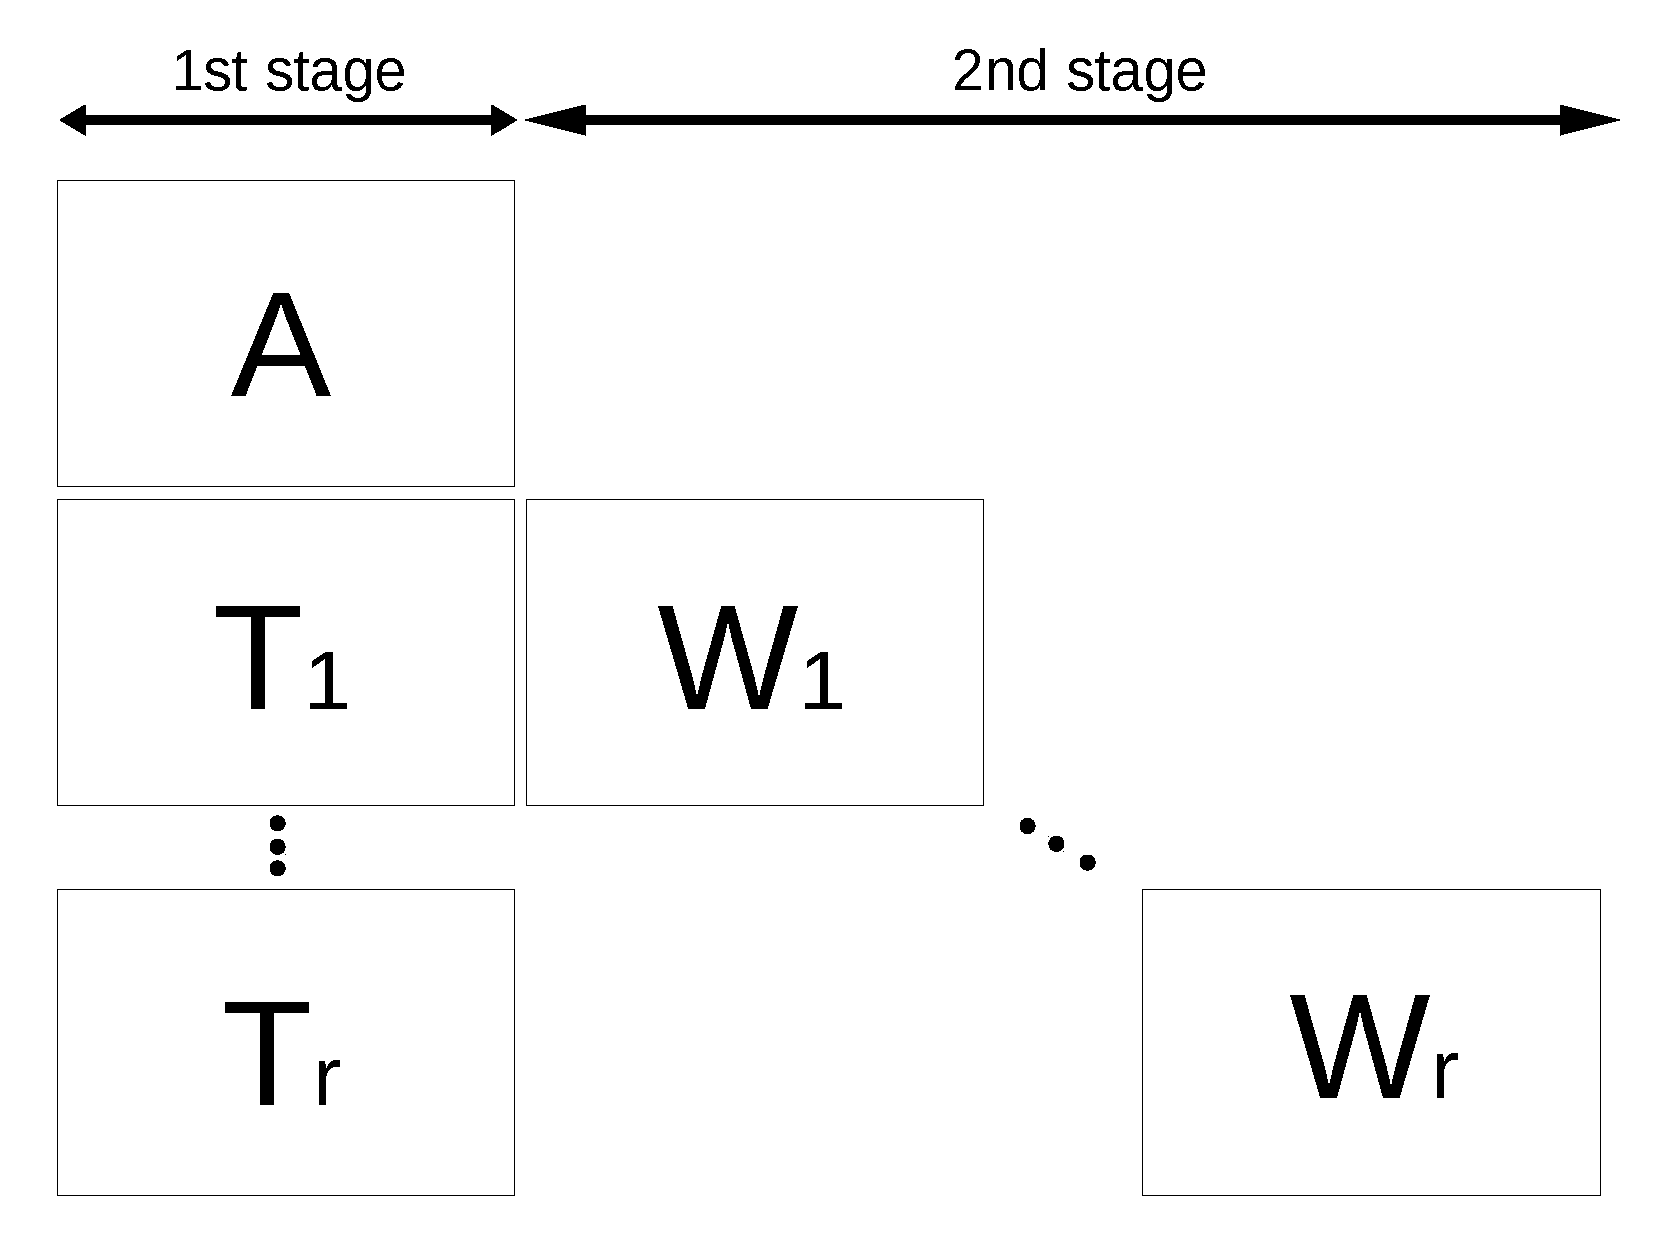
\includegraphics[width=0.5\linewidth]{drawings/stagewise_sparsity}
	\caption{Three (structurally) independent blocks in SIP}
	\label{fig:stagewise_sparsity}
\end{figure}
Associated with the blocks, every SIP in DEF has a block-diagonal structure in its coefficient matrix (Figure \ref{fig:de_structure}). This structure mainly differentiates SIP from the general MIP. In particular, the block-diagonal structure results always in high sparsity as scenario increases. Hence, it does not seem to be meaningful to just report the sparsity of coefficient matrix in DEF.
\begin{figure}[]
	\centering
	\subfloat[][AIRLIFT\_3]
	{
		\centering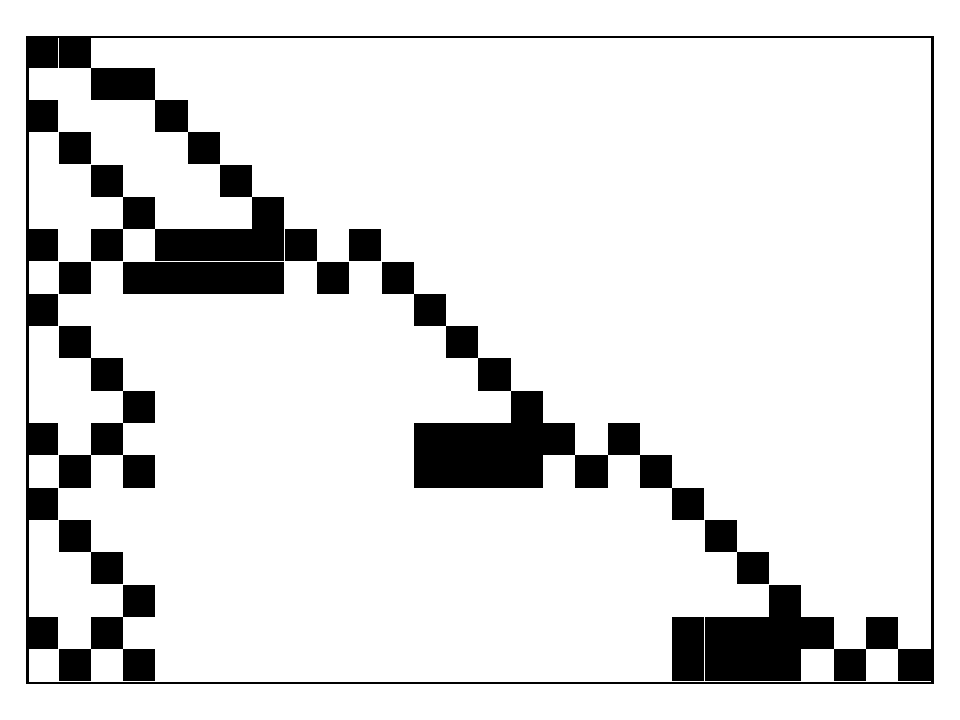
\includegraphics[width=0.31\linewidth]{AIRLIFT_3}
		\label{fig:de_structure_airlift}
	}
	~
	\subfloat[][CARGO\_3]
	{
		\centering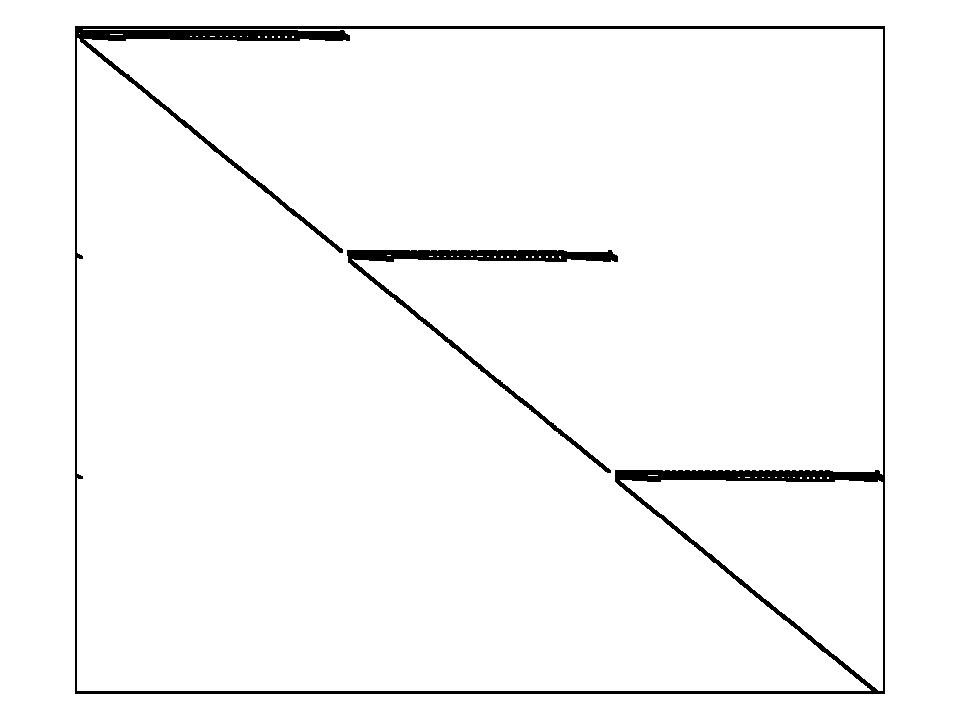
\includegraphics[width=0.31\linewidth]{CARGO_3}
		\label{fig:de_structure_cargo}
	}	
	~
	\subfloat[][CHEM\_3]
	{
		\centering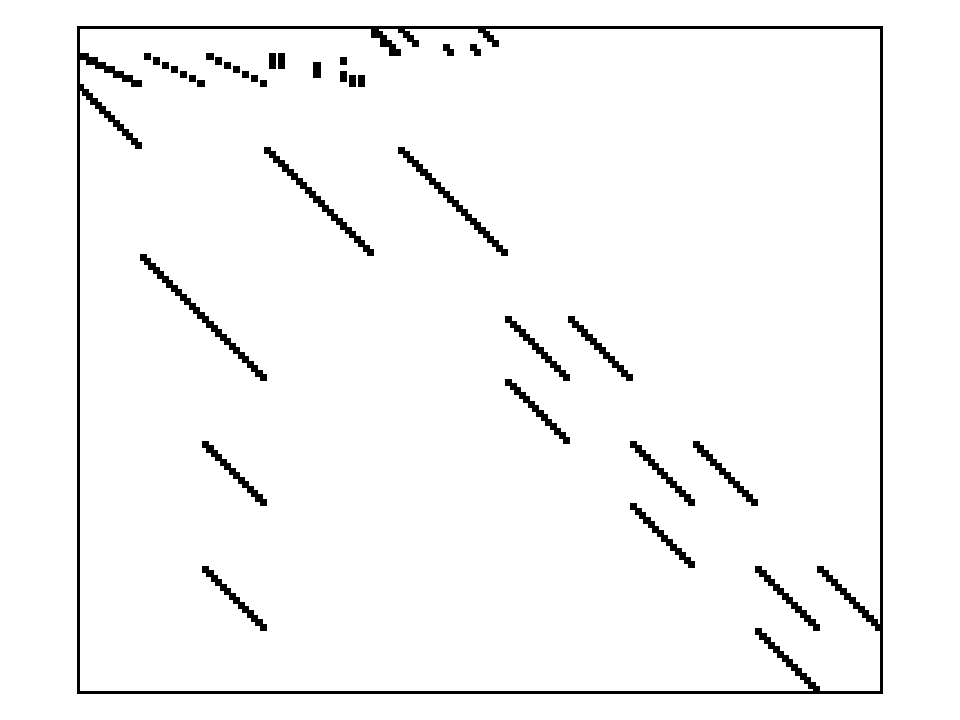
\includegraphics[width=0.31\linewidth]{CHEM_3}
		\label{fig:de_structure_chem}
	}		

	\subfloat[][DCAP\_3\_3\_3\_3]
	{
		\centering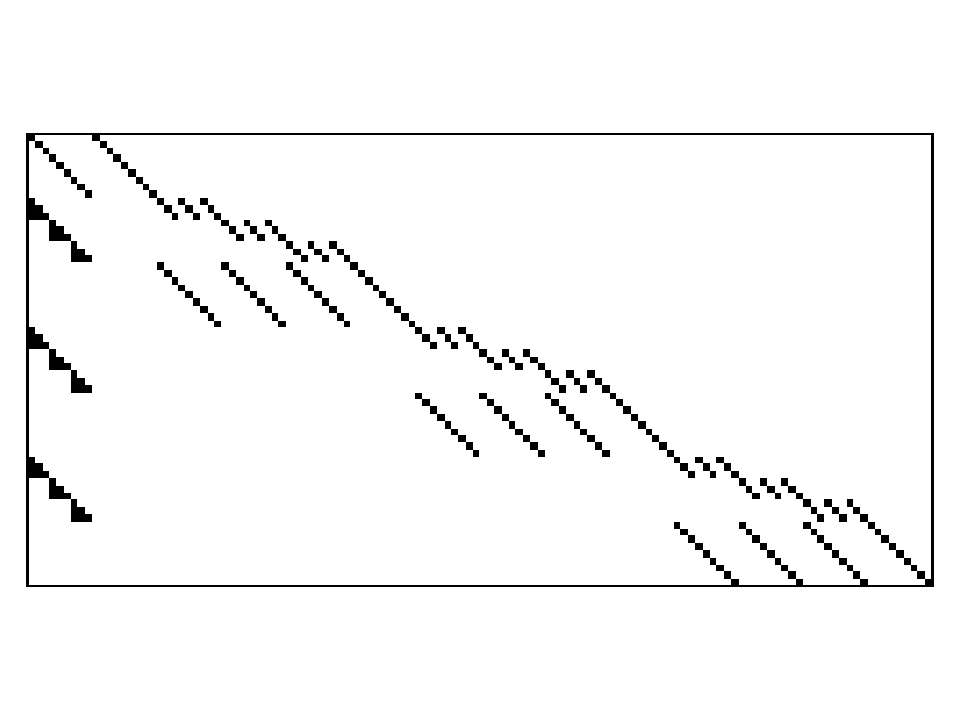
\includegraphics[width=0.31\linewidth]{DCAP_3_3_3_3}
		\label{fig:de_structure_dcap}
	}
	~	
	\subfloat[][MPTSPs\_D0\_3\_3]
	{
		\centering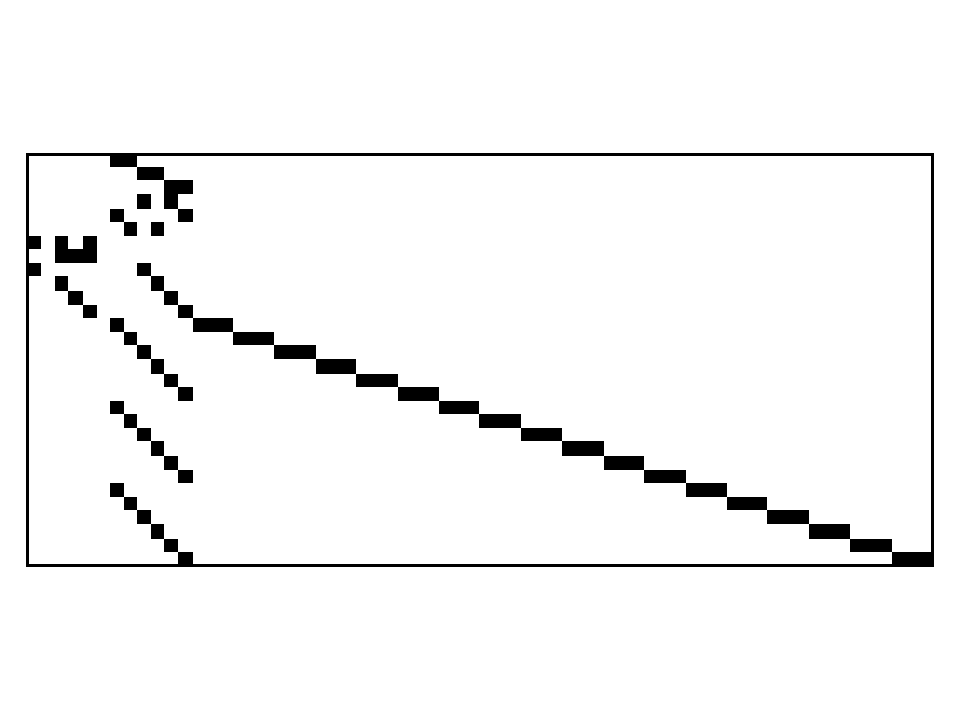
\includegraphics[width=0.31\linewidth]{MPTSPs_D0_3_3}
		\label{fig:de_structure_mptsps}
	}
	~
	\subfloat[][PHONE\_3]
	{
		\centering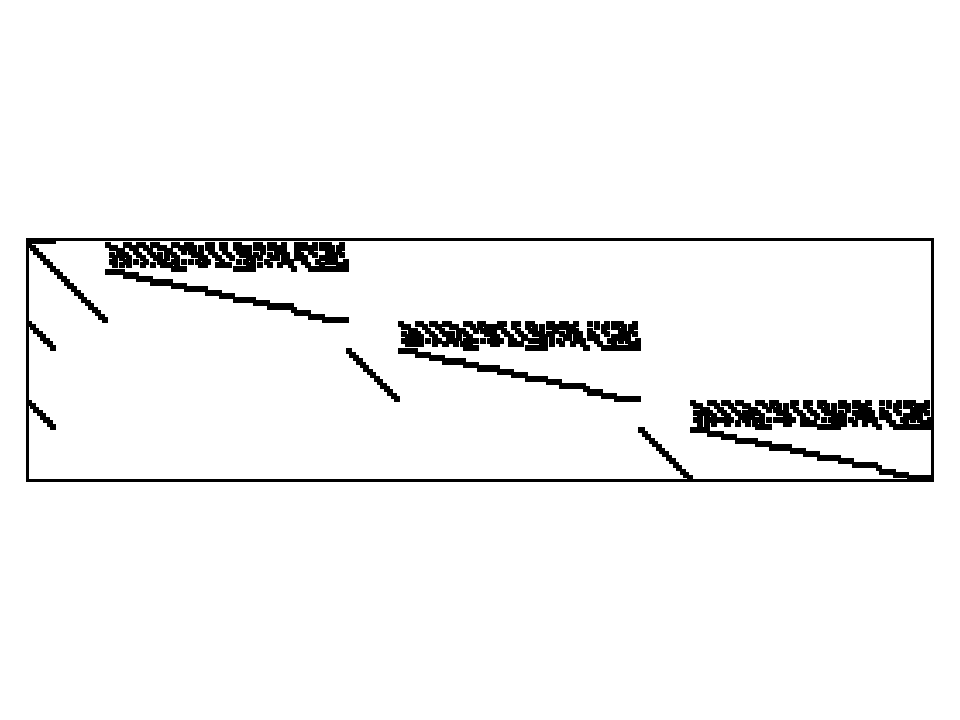
\includegraphics[width=0.31\linewidth]{PHONE_3}
		\label{fig:de_structure_mptsps}
	}
	
	\subfloat[][SDCP\_5\_10\_FallWD\_1]
	{
		\centering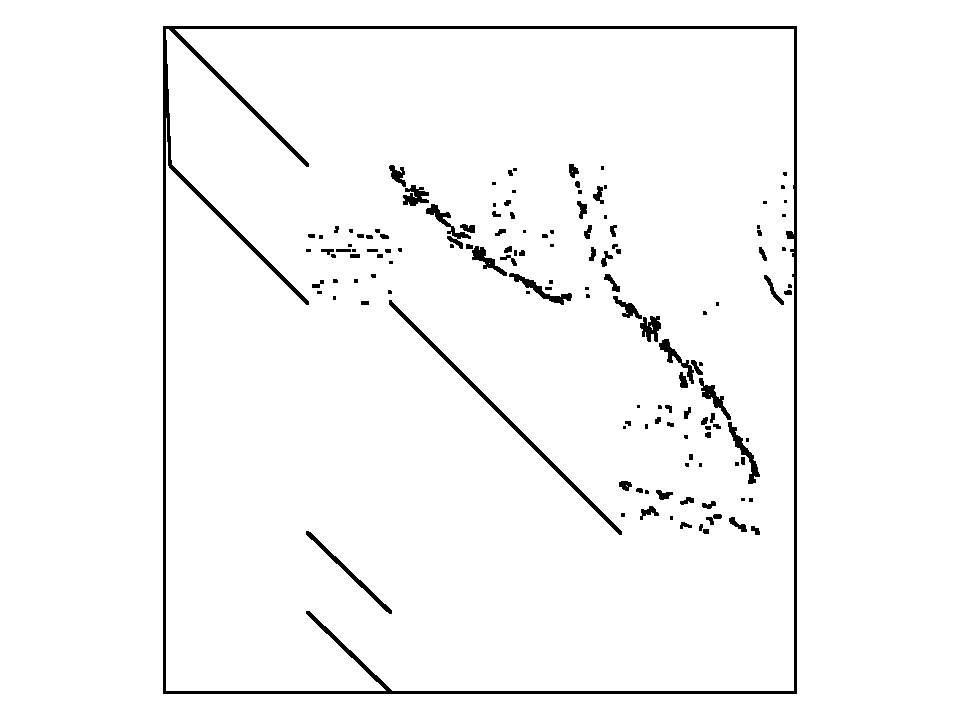
\includegraphics[width=0.31\linewidth]{SDCP_5_10_FallWD_1}
		\label{fig:de_structure_sdcp}
	}
	~	
	\subfloat[][SIZES\_3]
	{
		\centering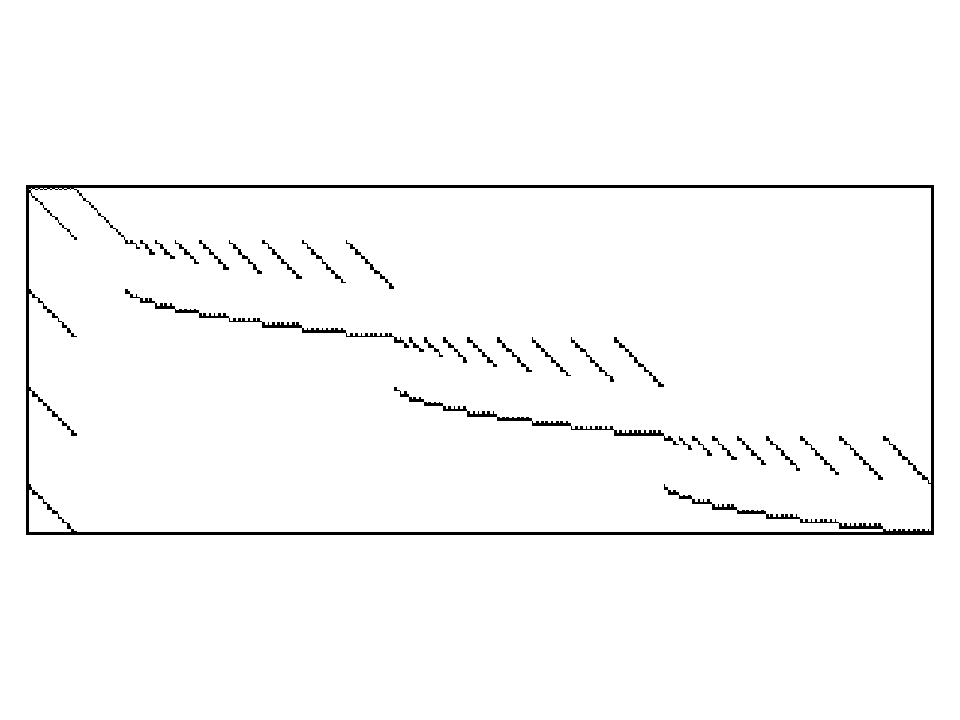
\includegraphics[width=0.31\linewidth]{SIZES_3}
		\label{fig:de_structure_sizes}
	}
	~
	\subfloat[][SMKP\_120\_3]
	{
		\centering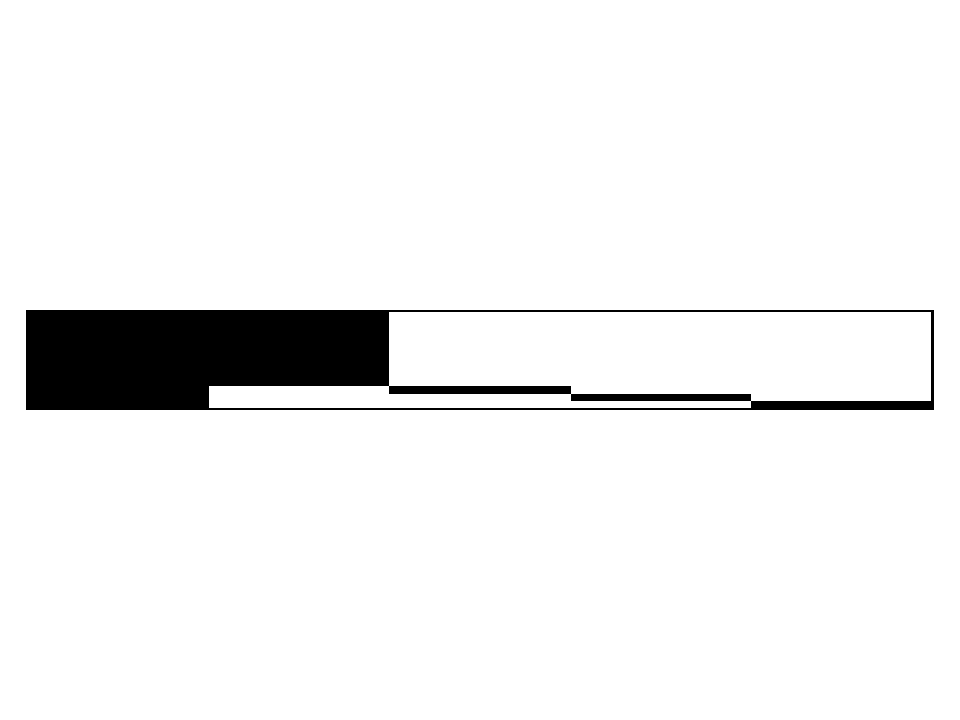
\includegraphics[width=0.31\linewidth]{SMKP_120_3}
		\label{fig:de_structure_smkp}
	}
	
	\subfloat[][SSLP\_5\_10\_3]
	{
		\centering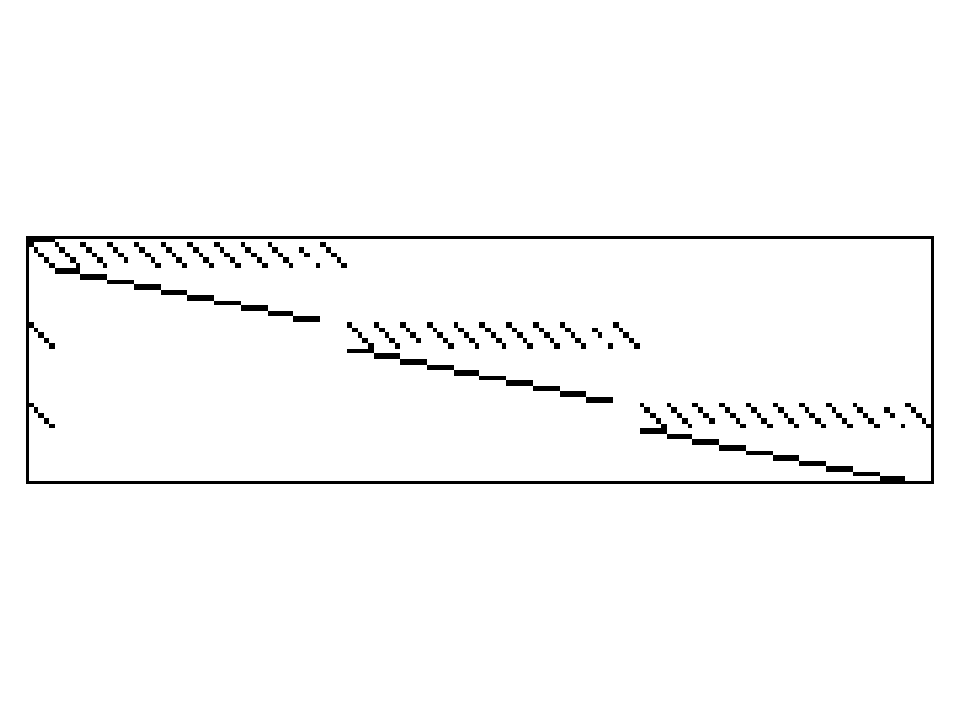
\includegraphics[width=0.45\linewidth]{SSLP_5_10_3}
		\label{fig:de_structure_sslp}
	}
	~
	\subfloat[][SUC\_FallWD\_1]
	{
		\centering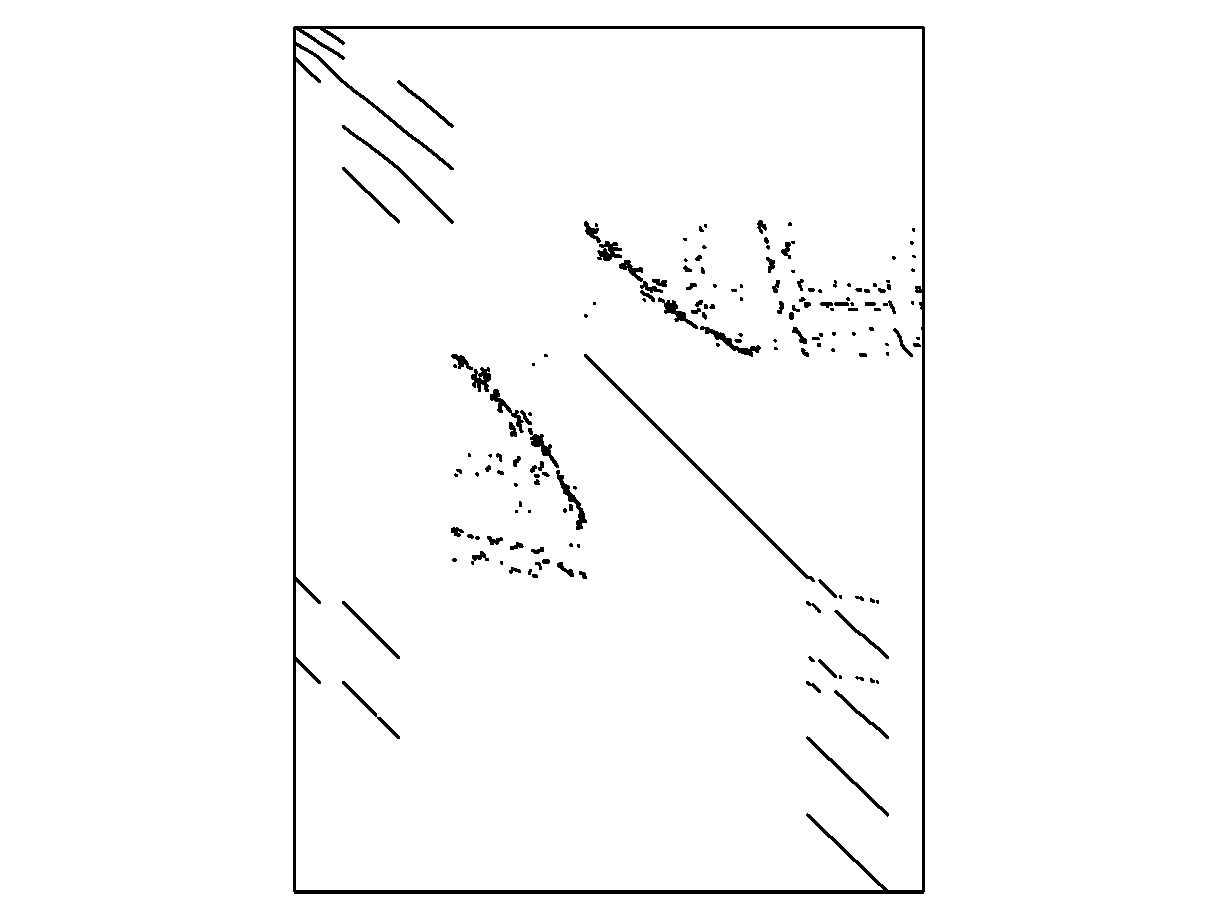
\includegraphics[width=0.45\linewidth]{SUC_FallWD_1}
		\label{fig:de_structure_sucw}
	}
	
	\caption{Block-diagonal structure in extensive form}
	%	\begin{minipage}
	%		{0.65\textwidth}{\footnotesize *\suc\ instance is too huge and extremely sparse to plot more than 1 scenario}
	%	\end{minipage}
	\label{fig:de_structure}
\end{figure}

As many decomposition-based methods in SIP make use of solution methods developed for MIP to solve the descendant master/sub problems, exploiting the sparsity pattern in each independent block might be one of the key factors that will help improving performance of the algorithms. For example, we would like to generate valid inequalities that preserve the sparse structure, intuitively. In that spirit, recent studies showed how well polytopes are approximated by using only sparse valid cuts \cite{journal:DMW2015,journal:DIM2015}.

%Low sparsity in matrices T and usually causes slowdown in decomposition algorithms. For example, the Dual Decomposition based solver \dsp\ shows much slower convergence speed than the centralized solver \cplex\ in problems like \smkp\ which always have low sparsity (nonzero ratio: 50\%-100\%, refer to Table \ref{table:sparsity_SMKP}).

%\kk{Would it be better to present the sparsity structure for one-scenario problem, like the one in .cor file?}
%\yoc{I tried to show the repeatedly duplicating patterns by looking at once. I think it would be good to add a subsection in section \ref{sec:prob_desc} to discuss problem-specific sparsity pattern for each problem and present the one-scenario instance sparsity pattern. }









